\documentclass[usenatbib,useAMS,usedcolumn]{mnras}

\usepackage{newtxtext,newtxmath}

% Use vector fonts, so it zooms properly in on-screen viewing software
% Don't change these lines unless you know what you are doing
\usepackage[T1]{fontenc}

% Allow "Thomas van Noord" and "Simon de Laguarde" and alike to be sorted by "N" and "L" etc. in the bibliography.
% Write the name in the bibliography as "\VAN{Noord}{Van}{van} Noord, Thomas"
\DeclareRobustCommand{\VAN}[3]{#2}
\let\VANthebibliography\thebibliography
\def\thebibliography{\DeclareRobustCommand{\VAN}[3]{##3}\VANthebibliography}

%%%%% AUTHORS - PLACE YOUR OWN PACKAGES HERE %%%%%

% Only include extra packages if you really need them. Common packages are:
\usepackage{graphicx}	% Including figure files
\graphicspath{{fig/}}
\usepackage{amstext}
\usepackage{siunitx}
\sisetup{
separate-uncertainty,  
range-units = brackets}  
\usepackage{mathtools}
\usepackage{color}
\usepackage{twoopt}
\usepackage{hyperref} %% to avoid \citeads line fills
\usepackage{afterpage}
\usepackage{silence}
\usepackage{hyperref}
\usepackage{anyfontsize}

%%%%%%%%%%%%%%%%%%%%%%%%%%%%%%%%%%%%%%%%%%%%%%%%%%

%%%%% AUTHORS - PLACE YOUR OWN COMMANDS HERE %%%%%

% common astronomical symbols
\let\sun\odot
% astrophysical units
\DeclareSIUnit\lightspeed{$c$}
\DeclareSIUnit\rydberg{Ry}
\DeclareSIUnit\erg{erg}
\DeclareSIUnit\magnitude{mag}
\DeclareSIUnit\jansky{Jy}
\DeclareSIUnit\gauss{G}
\DeclareSIUnit\h{$h$}
\DeclareSIUnit\hseven{$h$_7}
\DeclareSIUnit\parsec{pc}
\DeclareSIUnit\year{yr}
\DeclareSIUnit\solarluminosity{\ensuremath{L_\sun}}
\DeclareSIUnit\solarmass{\ensuremath{M_\sun}}
\DeclareSIUnit\solarmassinenergy{\ensuremath{M_\sun|c^2}}
\DeclareSIUnit\solarradius{\ensuremath{R_\sun}}
% redeclared units
\DeclareSIUnit\arcsecond{as}
\DeclareSIUnit\astronomicalunit{au}
\DeclareSIUnit\clight{\ensuremath c}

% Please keep new commands to a minimum, and use \newcommand not \def to avoid
% overwriting existing commands. Example:
%\newcommand{\pcm}{\,cm$^{-2}$}	% per cm-squared

\bibpunct{(}{)}{;}{a}{}{,}             %% natbib format for A&A and ApJ
\makeatletter
  \newcommandtwoopt{\citeads}[3][][]{\href{http://adsabs.harvard.edu/abs/#3}%
    {\def\hyper@linkstart##1##2{}%
     \let\hyper@linkend\@empty\citealp[#1][#2]{#3}}}
  \newcommandtwoopt{\citepads}[3][][]{\href{http://adsabs.harvard.edu/abs/#3}%
    {\def\hyper@linkstart##1##2{}%
     \let\hyper@linkend\@empty\citep[#1][#2]{#3}}}
  \newcommandtwoopt{\citetads}[3][][]{\href{http://adsabs.harvard.edu/abs/#3}%
    {\def\hyper@linkstart##1##2{}%
     \let\hyper@linkend\@empty\citet[#1][#2]{#3}}}
  \newcommandtwoopt{\citeyearads}[3][][]%
    {\href{http://adsabs.harvard.edu/abs/#3}
    {\def\hyper@linkstart##1##2{}%
     \let\hyper@linkend\@empty\citeyear[#1][#2]{#3}}}
%  \renewcommand*\aa@pageof{, page \thepage{} of \pageref*{LastPage}}
\makeatother
\hypersetup{pdfpagemode = {UseNone},
            pdftitle = {The dispersal of protoplanetary discs},
            pdfcreator = {\LaTeX},
            pdfproducer = {pdfeTeX-0.\the\pdftexversion\pdftexrevision},
            pdfauthor = {Giovanni Picogna, Barbara Ercolano, Catherine Espaillat},
            pdfsubject = {},
            pdfview = {FitH},
            pdfstartview = {FitH},
            colorlinks = {true},
            linkcolor = [rgb]{0,0.35,0.7},
            citecolor = [rgb]{0,0.35,0.7},
            filecolor = [rgb]{0.61,0,0},
            urlcolor = [rgb]{0,0.35,0.7},
           }

\WarningFilter{latex}{Text page}

\newcommand{\new}[1]{{\bf \color{black} #1}}
\newcommand{\todo}[1]{{\bf \color{red} #1}}

\defcitealias{2019MNRAS.487..691P}{Paper~I}
\defcitealias{2021MNRAS.508.1675E}{Paper~II}
\defcitealias{2021MNRAS.508.3611P}{Paper~III}

%%%%%%%%%%%%%%%%%%%%%%%%%%%%%%%%%%%%%%%%%%%%%%%%%%

%%%%%%%%%%%%%%%%%%% TITLE PAGE %%%%%%%%%%%%%%%%%%%

% Title of the paper, and the short title which is used in the headers.
% Keep the title short and informative.
\title[The dispersal of protoplanetary discs]{The dispersal of protoplanetary discs. -- IV: Influence of gas cavity on disc photoevaporation}

% The list of authors, and the short list which is used in the headers.
% If you need two or more lines of authors, add an extra line using \newauthor
\author[G. Picogna et al.]{
   Giovanni Picogna,$^{1}$ \href{https://orcid.org/0000-0003-3754-1639}{
\includegraphics[scale=0.04]{orcid}} \thanks{E-mail: picogna@usm.lmu.de}
   Kristina Monsch,$^{3}$ \href{https://orcid.org/0000-0002-5688-6790}{
\includegraphics[scale=0.04]{orcid}}
   Ercolano Barbarao$^{1,2}$ \href{https://orcid.org/0000-0001-7868-2740}{
\includegraphics[scale=0.04]{orcid}}
\\
% List of institutions
$^{1}$Universit\"{a}ts-Sternwarte, Ludwig-Maximilians-Universit\"{a}t M\"{u}nchen,
        Scheinerstr. 1, D-81679 M\"{u}nchen, Germany\\
$^{2}$Excellence Cluster Origins, Boltzmannstrasse 2, D-85748 Garching bei M\"{u}nchen, Germany\\
$^{3}$Department of Astronomy \& Institute for Astrophysical Research, Boston University, 725 Commonwealth Avenue, Boston, MA 02215, USA
}

% These dates will be filled out by the publisher
\date{Accepted XXX. Received YYY; in original form ZZZ}

% Enter the current year, for the copyright statements etc.
\pubyear{2021}

% Don't change these lines
\begin{document}
\label{firstpage}
\pagerange{\pageref{firstpage}--\pageref{lastpage}}
\maketitle

% Abstract of the paper
\begin{abstract}
The strong X-ray irradiation from young solar-type stars may play a crucial role in the thermodynamics and chemistry of circumstellar discs, driving their evolution in the last stages of disc dispersal as well as shaping the atmospheres of newborn planets.
In this paper we study the influence of stellar mass on circumstellar disc mass-loss rates due to X-ray irradiation, extending our previous study of the mass-loss rate's dependence on the X-ray luminosity and spectrum hardness. We focus on stars with masses between $0.1$ and \SI{1}{\solarmass}, which are the main target of current and future missions to find potentially habitable planets.
We find a linear relationship between the mass-loss rates and the stellar masses when changing the X-ray luminosity accordingly with the stellar mass.
This linear increase is observed also when the X-ray luminosity is kept fixed because of the lower disc aspect ratio which allows the X-ray irradiation to reach larger radii.
We provide new analytical relations for the mass-loss rates and profiles of photoevaporative winds as a function of the stellar mass that can be used in disc and planet population synthesis models.
Our photoevaporative models correctly predict the observed trend of inner-disc lifetime as a function of stellar mass with an increased steepness for stars smaller than \SI{0.3}{\solarmass}, indicating that X-ray photoevaporation is a good candidate to explain the observed disc dispersal process.
\end{abstract}

% Select between one and six entries from the list of approved keywords.
% Don't make up new ones.
\begin{keywords}
    accretion, accretion discs --
    protoplanetary discs --
    circumstellar matter --
    stars: pre-main-sequence --
    stars: winds, outflows --
    X-rays: stars.
\end{keywords}

%%%%%%%%%%%%%%%%%%%%%%%%%%%%%%%%%%%%%%%%%%%%%%%%%%

%%%%%%%%%%%%%%%%% BODY OF PAPER %%%%%%%%%%%%%%%%%%

%-------------------------------------------------------------------
\section{Introduction}
%-------------------------------------------------------------------

Our understanding of the physical processes driving the evolution of protoplanetary discs and ultimately the formation of planets is based on the observational evidence of disc lifetimes.
\citetads{1989AJ.....97.1451S} found that accretion discs are ubiquitous around young stellar objects (\SI{\sim 1}{Myr}). The initial disc fraction is almost independent of stellar mass (from $0.1$ up to \SI{10}{\solarmass}) and stellar environment (\citeads{2000AJ....120.3162L}, \citeads{2006A&A...451..177B}).
After \SI{10}{Myr} the picture changes completely since more than \SI{90}{\percent} of stars show no emission within \SI{1}{\astronomicalunit} \citepads{2004ApJ...612..496M}, and emission from small grains is found only in a few per cent of discs (\citeads{2004ApJ...608..526L}, \citeads{2005AJ....129.1049C}, \citeads{2006ApJ...639.1138S}).
This sets an upper limit to the disc dispersal process within $10$ to \SI{20}{Myr} (\citeads{2007ApJ...671.1784H}, \citeads{2010A&A...510A..72F}, \citeads{2014A&A...561A..54R}). Moreover, fitting the fraction of discs with dust emission at different wavelengths, \citetads{2014A&A...561A..54R} found an e-folding time of \SIrange{2}{3}{Myr} at \SIrange[]{3}{12}{\micro\meter} and \SIrange[]{4}{6}{\mega\year} at \SIrange[]{22}{24}{\micro\meter}, hinting at an inside-out dispersal of proto-planetary discs or to a second generation dust production \citepads[see also][]{2013MNRAS.428.3327K}.
The dust disc lifetime as a function of the stellar mass is less well characterised but the dispersal timescale appears to be up to two times faster for high mass stars ($\geq$ \SI{2}{\solarmass}, \citeads{2015A&A...576A..52R}).
The mass accretion onto the central star has also been studied extensively, though its evolution is less well constrained. Nevertheless, it has been shown that the characteristic timescale of disc accretion is shorter than that of dust disc dispersal (\citeads{2006ApJ...648.1206J}, \citeads{2010A&A...510A..72F}), and the accretion rate falls off as a function of time with a power law (e.g., \citeads{2012ApJ...755..154M}, \citeads{2014A&A...572A..62A}, \citeads{2016ARA&A..54..135H}).

The main physical process driving disc dispersal is still largely unconstrained, and it might change during the disc evolution and at different locations in the disc. A large body of evidence is pointing at magnetic disc winds as the main mechanism responsible for angular momentum transfer and mass-loss \citepads{2016ApJ...821...80B}, particularly at early times. Photoevaporative disc winds may also co-exist at early times and perhaps dominate at later stages (\citeads{2017RSOS....470114E}; \citeads{2020MNRAS.496..223W}). From a theoretical standpoint, there is a push to obtain better models that can be linked to observables to test their validity.

In the first paper of this series (\citeads{2019MNRAS.487..691P}, hereafter \citetalias{2019MNRAS.487..691P}) we showed the dependence between the stellar X-ray luminosity and the mass-loss rate due to thermal winds generated by the XEUV heating from the central star. Then we studied the influence of carbon depletion \citepads{2019MNRAS.490.5596W} and stellar spectra hardness on the mass-loss rates (\citeads{2021MNRAS.508.1675E}, hereafter \citetalias{2021MNRAS.508.1675E}). Finally we looked in the dependance of mass-loss rate and stellar mass (\citeads{2021MNRAS.508.3611P}, hereafter \citetalias{2021MNRAS.508.3611P}). In this following work, we bring all the previous results together, and study the influence of the gap hole radii dependance and the implications to interprete current and future observations of transition discs.

In Section~\ref{sec:methods} we briefly discuss the numerical set-up adopted, following our previous work. We then describe the main results in Section~\ref{sec:results} and discuss their theoretical and observational implications in Section~\ref{sec:discussion}. The main conclusions are then drawn in Section~\ref{sec:conclusions}.

%-------------------------------------------------------------------
\section{Methods}\label{sec:methods}
%-------------------------------------------------------------------
We run a series of hydrodynamical simulations following the approach outlined in \citetalias{2019MNRAS.487..691P} that we briefly describe here for completeness.

The initial set-up is based on the gas densities and dust temperatures from the hydrostatic disc models from the D’Alessio Irradiated Accretion Disk (\textsc{diad}) radiative transfer models \citepads{1998ApJ...500..411D,1999ApJ...527..893D,2001ApJ...553..321D,2005ApJ...621..461D,2006ApJ...638..314D}, that best fit the median spectral energy distribution (SED) in Taurus. 
For this particular study a different set-up is adopted for each individual stellar mass, based on its mass and bolometric luminosity.
The stellar parameters were obtained from \citetads{2000A&A...358..593S} for an age of \SI{1}{Myr}, and a metallicity $Z=0.02$ without overshooting.

We then ran the gas photoionization and dust radiative transfer code \textsc{mocassin} \citepads{2003MNRAS.340.1136E,2005MNRAS.362.1038E,2008ApJS..175..534E}, that solves the heating and cooling terms for various physical and irradiation properties at thermal equilibrium, to obtain a temperature prescription in the upper layers of the discs when irradiated by an X(EUV) stellar spectrum.
We adopted X-ray luminosities scaled as a function of stellar mass following \citetads{2007A&A...468..353G}
\begin{equation}\label{eq:Lx}
	\log_{10}{(\mathrm{L}_X)} = (1.54 \pm 0.12) \log_{10}{(\mathrm{M}_\star)} + (30.31 \mp 0.06)\,,
\end{equation}
although a recent analysis by \citetads{2021A&A...648A.121F} found a steeper dependence.

The temperature prescription changes for the different spectral hardness (from \texttt{Spec29} corresponding to \SI{e29}{erg.s^{-1}} to \texttt{Spec31} equal to \SI{e31}{erg.s^{-1}}) following \citetalias{2021MNRAS.508.1675E}.
It relates the local gas temperature to the column density to the central star (from \SI{5e20}{pp.cm^{-2}} to \SI{2e22}{pp.cm^{-2}}), and the local ionization parameter \citepads{1969ApJ...156..943T}
\begin{equation}
    \xi = \frac{L_X}{n r^2}\,,
\end{equation}
where $L_X$ is the X-ray luminosity, $n$ the number density, and $r$ the spherical radius from the central star. We compared it for completeness with the previously derived temperature prescription (used in \citetalias{2019MNRAS.487..691P}) obtained for a star with $L_X=\SI{2e30}{erg.s^{-1}}$ in \citetads{2008ApJS..175..534E}.

Finally we ran a set of hydrodynamical simulations with a modified version of the \textsc{pluto} code \citepads{2007ApJS..170..228M} presented in \citetalias{2019MNRAS.487..691P}, in order to use the temperature prescription from \textsc{mocassin} for column densities lower than the maximum penetration depth of X-rays (\SI{\sim 2e22}{pp.cm^{-2}}), and a perfect coupling between gas and dust temperatures using the \textsc{diad} models for larger column densities.
We evolve the models until a steady state is reached for the disc structure and the gas streamlines in the wind.

We modelled $4$ different stellar masses, ranging from \SI{0.1}{\solarmass} to \SI{1}{\solarmass} which, together with the \SI{0.7}{\solarmass} studied in \citetalias{2019MNRAS.487..691P}, allow us to study in detail the stellar mass dependence on the mass-loss rates due to photoevaporative winds in T Tauri stars. The initial parameters adopted in the different runs are summarised in Table~\ref{tab:stars}.

\begin{table*}
\caption{Stellar properties}
\label{tab:stars}
\centering
\begin{tabular}{c c c c c c c c}
\hline
Name & $\mathrm{M}_\star$ [\si{\solarmass}] & $\mathrm{R}_\star$ [\si{\solarradius}] & ST & $\mathrm{L}_\star$ [\si{\solarluminosity}] & $\mathrm{L}_X$ [\SI{e29}{erg.s^{-1}}] & $\mathrm{T}_\star$ [\si{\kelvin}] & Spectrum\\
\hline
\hline
   \texttt{1Msun} & $1.0$ & $2.615$ & K6 & $2.335$ & $20.4$ & $4278$ & $\texttt{Spec30}$ \\
   \texttt{0.5Msun} & $0.5$ & $2.125$ & M1 & $0.9288$ & $7.02$ & $3771$ & $\texttt{Spec30}$ \\
   \texttt{0.3Msun} & $0.3$ & $2.310$ & M5 & $0.6887$ & $3.20$ & $3360$ & $\texttt{Spec29}$ \\
   \texttt{0.1Msun} & $0.1$ & $1.055$ & M6 & $0.0856$ & $0.59$ & $2928$ & $\texttt{Spec29}$ \\
\hline
\end{tabular}
\end{table*}

\subsection{Hydrodynamical model}\label{sec:hydro-model}

We adopted a spherical coordinate system centred on the star.
The grid is logarithmically spaced in the radial direction with \SI{500}{cells}, in order to have better resolution in the inner region of the disc, where photoevaporation is mostly effective.
At the same time, it allows us to model the disc out to large radii (R$_\mathrm{out}$ = \SI{600}{\astronomicalunit}) without strongly increasing our computational costs and preventing boundary effects that can affect the stability of the wind flow.
For a detailed discussion of the numerical artefacts induced by the grid outer boundary, the reader is referred to \citetalias{2019MNRAS.487..691P}.
The grid is spaced linearly in the polar direction, with a refinement at the wind launching region (\SI{100}{cells} from $0.01$ to \SI{0.5}{rad}, \SI{200}{cells} from $0.5$ to \SI{1}{rad}, and $50$ cells from $1$ to $\pi / 2$ rad).

We evolve the system between 500 and 1000 orbits at \SI{10}{au} with stellar irradiation (applied through a parameterisation as explained above and in \citetalias{2019MNRAS.487..691P}) until the cumulative mass-loss rate and gas streamline in the wind have reached a steady-state after few hundred orbital periods (at \SI{10}{au}). We also double the resolution for few of the test runs to check that we are capturing the proper physical scales.

%-------------------------------------------------------------------
\section{Results}\label{sec:results}
%-------------------------------------------------------------------

\subsection{Disc profiles}

\begin{figure*}
   \centering
   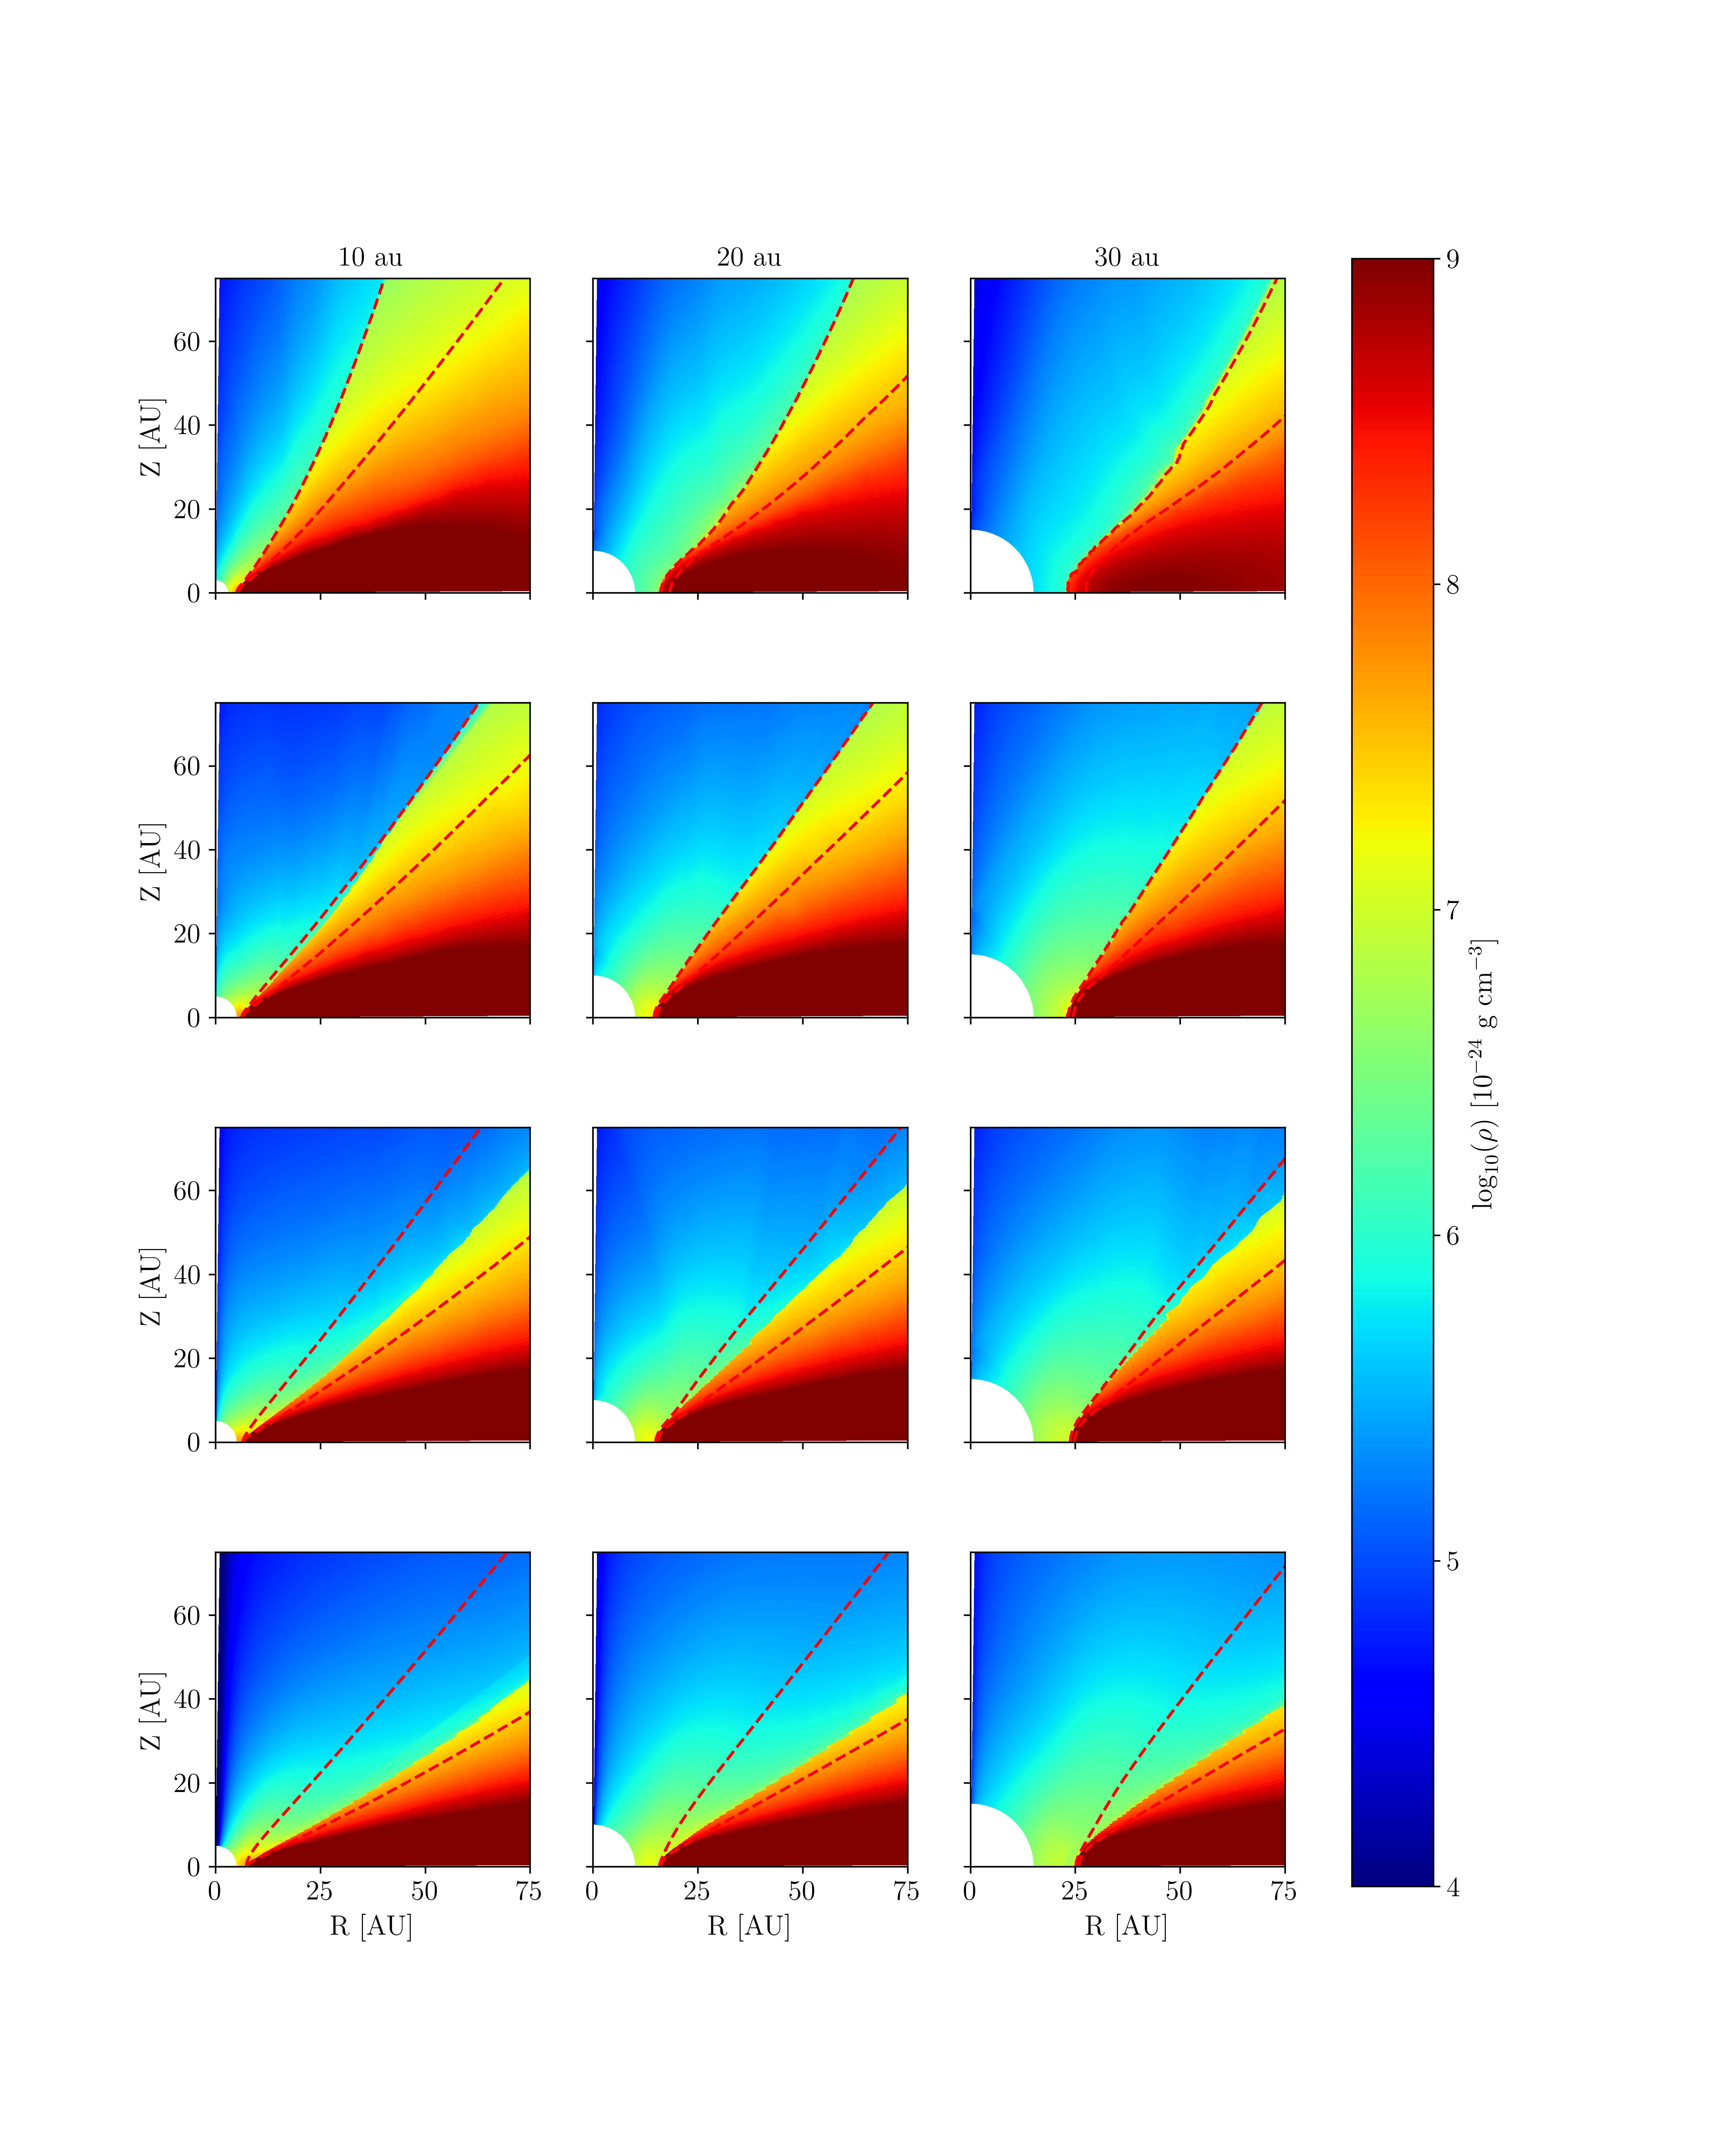
\includegraphics[width=\textwidth]{CompHoles}
   \caption{Gas density averaged over 10 orbits after 500 orbits (at 10 au) for the different stellar masses and gap radii. The column densities at $5e20$ and $1e22$, representing the maximum penetration depth of EUV and X-rays are overplotted with red dashed lines. \label{fig:2Ddensdiscs}}
\end{figure*}

\subsection{Mass-loss rates}\label{sec:mdot}

\begin{figure}
   \centering
   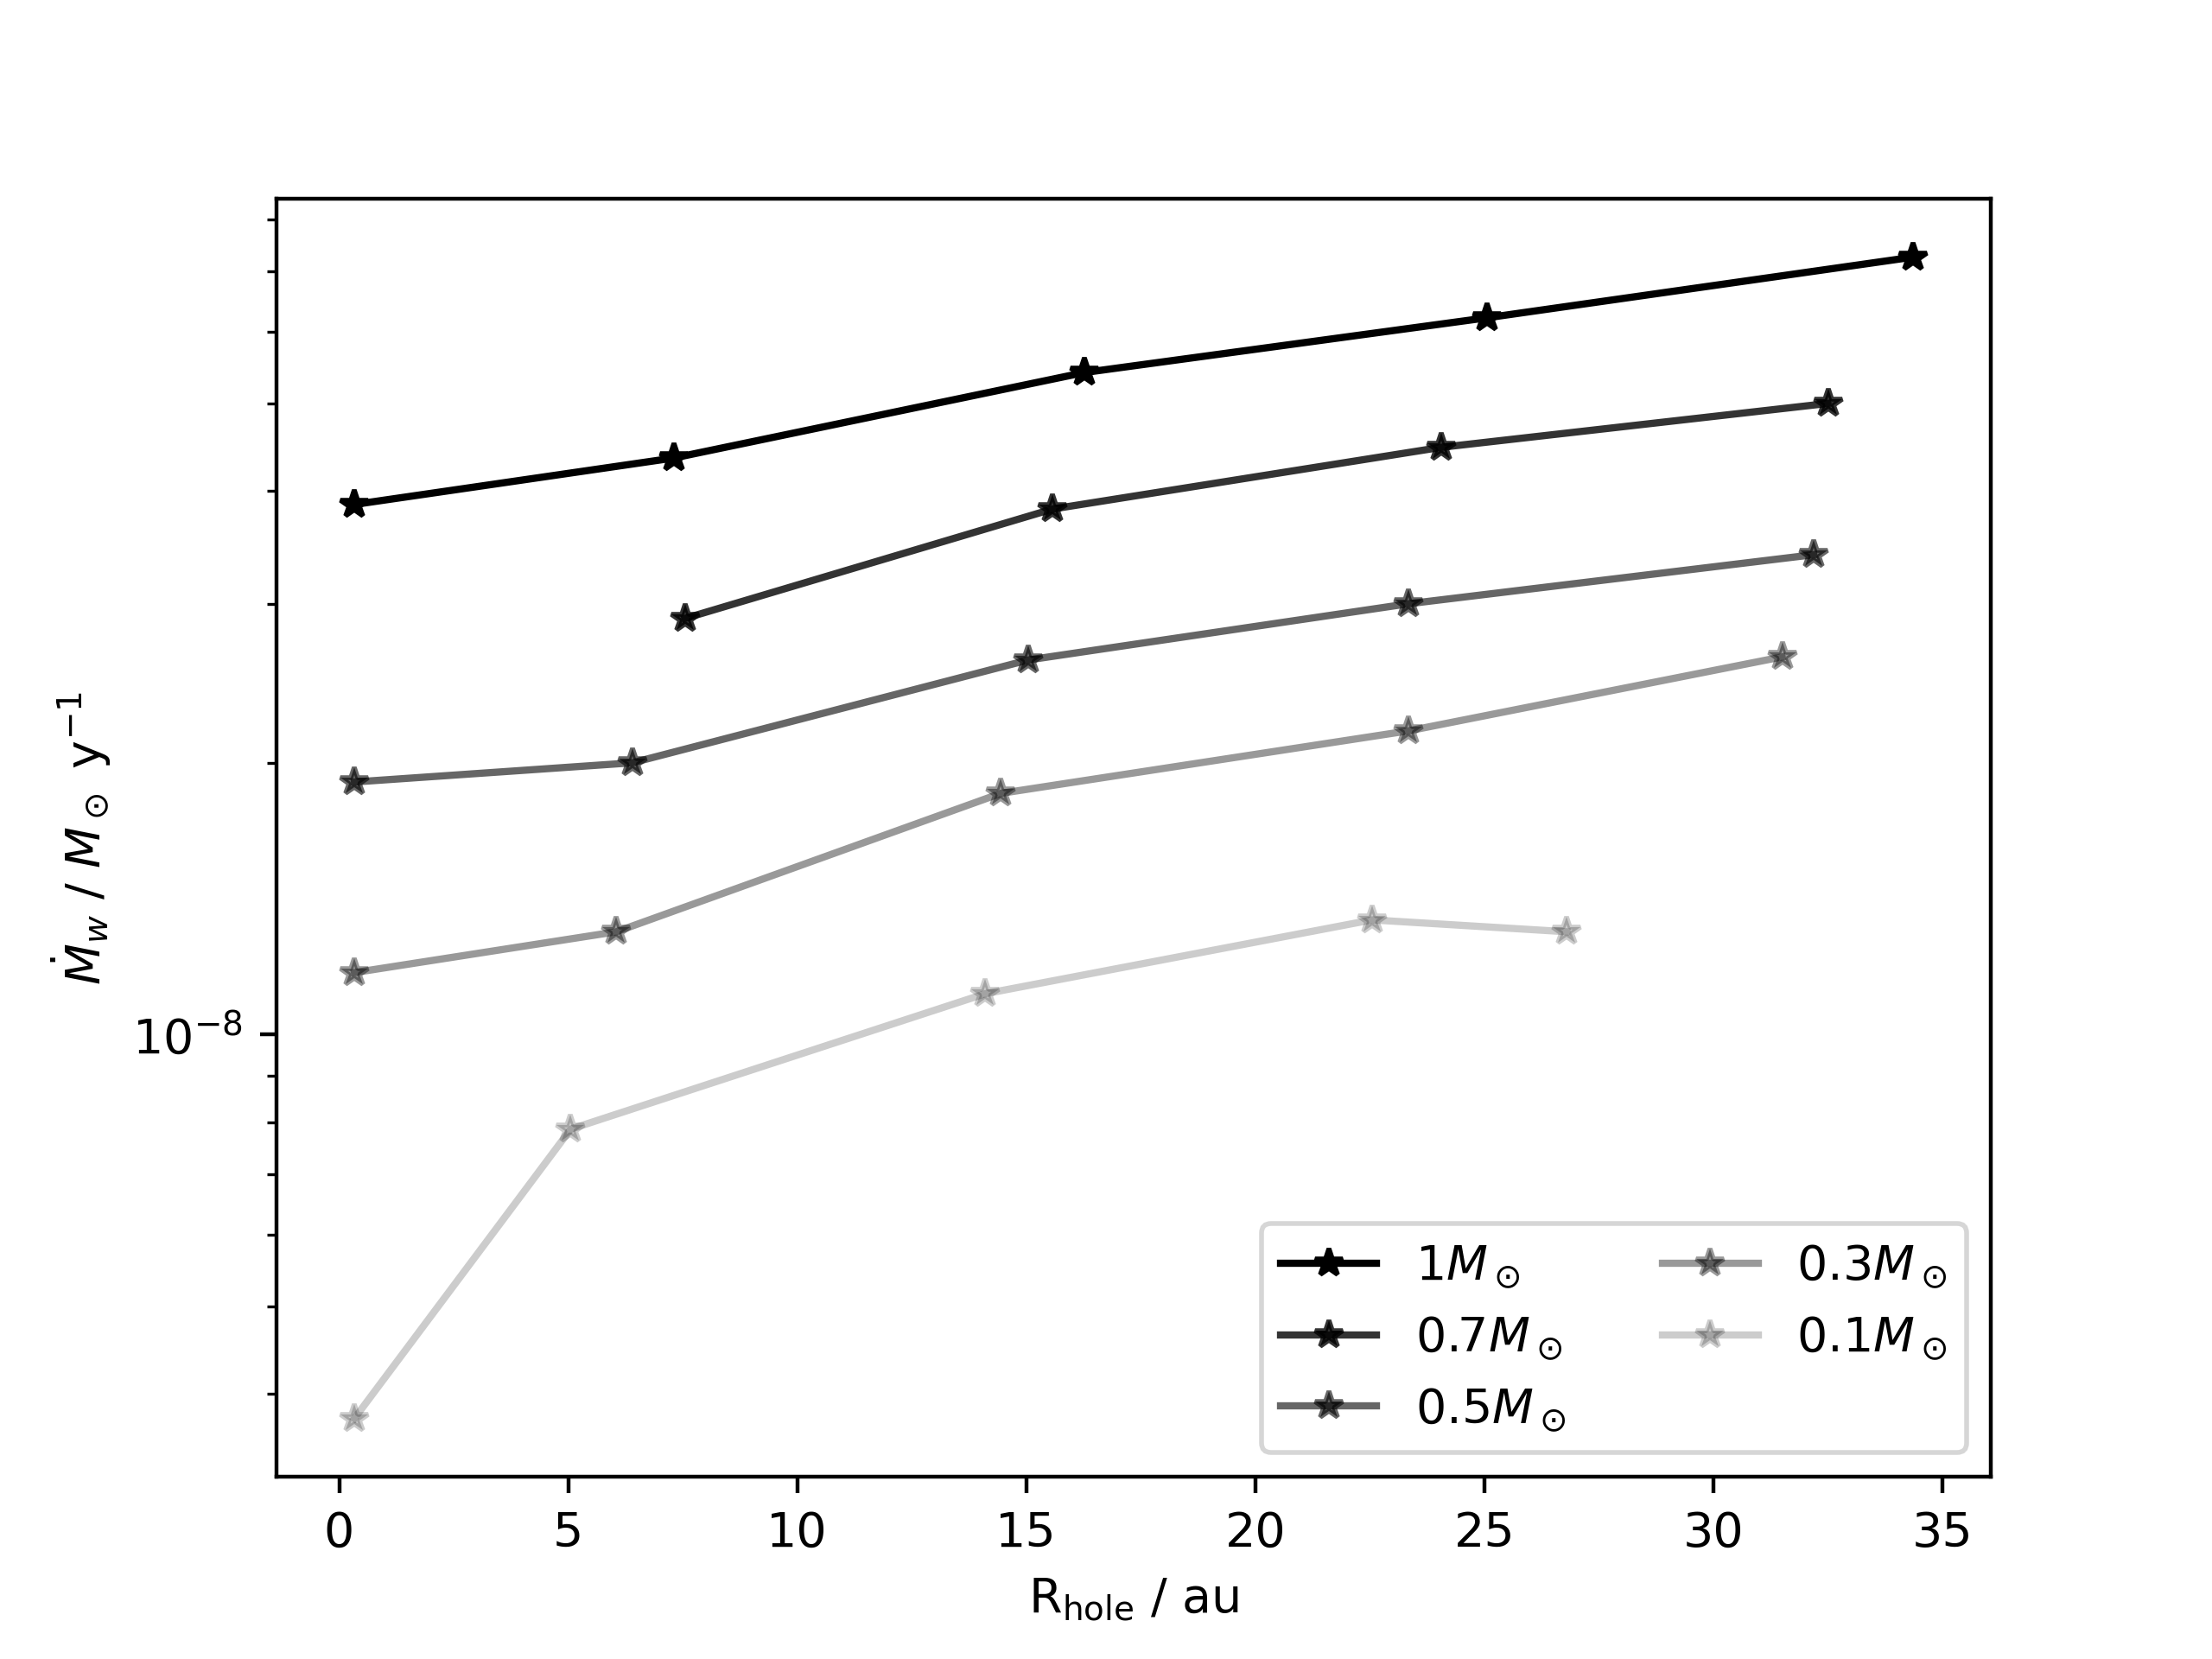
\includegraphics[width=0.5\textwidth]{Mdot.png}
   \caption{Cumulative mass-loss rate as a function of gap cavity for different stellar masses.
   \label{fig:mdot}}
\end{figure}

\begin{figure}
   \centering
   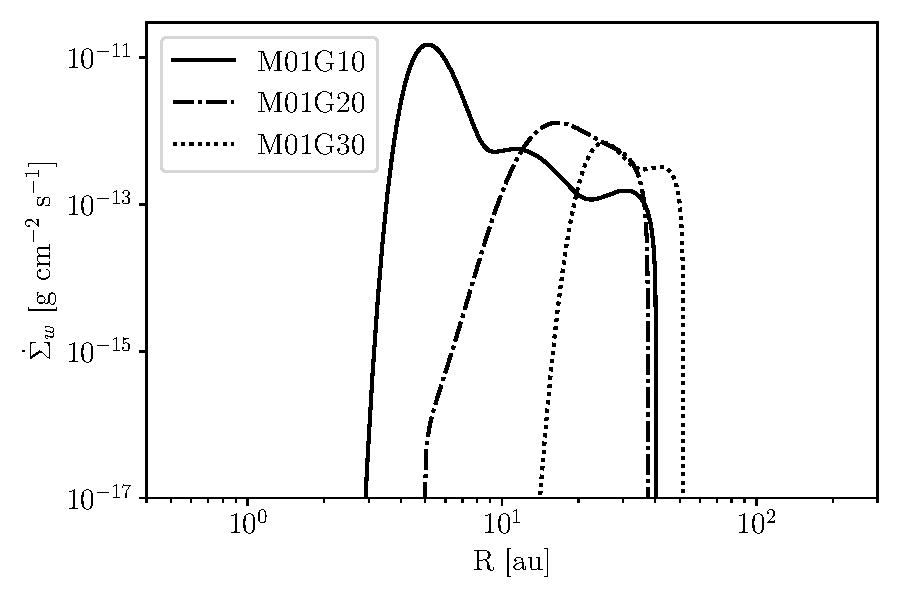
\includegraphics[width=0.5\textwidth]{Sigmadot01}
   \caption{Surface mass-loss rate as a function of the cylindrical distance from the central star of \SI{0.1}{\solarmass} and initial gap holes of $10$, $20$, $30$ au respectively. 
   \label{fig:Sigmadot01}}
\end{figure}

\subsection{Wind profiles}\label{sec:wind-prof}

\subsection{Gas cavity radius dependence}\label{sec:gap-dependance}

%-------------------------------------------------------------------
\section{Discussion}\label{sec:discussion}
%-------------------------------------------------------------------

\subsection{Comparison with observations}

\begin{itemize}
   \item compare population synthesis with observations of transition discs with gap in the gas component
   \item extend analysis previous paper to more star forming regions both with analytical approach and pop-synthesis
   \item what is the evolution of the surface density of discs where PE is taking place?
\end{itemize}

\subsection{Comparison with other models}

\begin{itemize}
   \item what is the fraction of systems where photoevaporation might be the primary cause of gap opening
   \item which part of the parameter space is covered by planets/MHD winds?
   \item what is the role of external photoevaporation?
\end{itemize}

%-------------------------------------------------------------------
\section{Conclusions}\label{sec:conclusions}
%-------------------------------------------------------------------

  We have computed for the first time comprehensive photoevaporation models spanning the whole observed range of low mass stars ($\leq$ \SI{1}{\solarmass}) and gas cavity radii using observationally derived X-ray stellar spectra. 
  We found that

   \begin{enumerate}
      \item  
   \end{enumerate}

\section{Data availability}
   The data underlying this article and the scripts used to create the Figures are available at \href{https://cutt.ly/9XlQTGV}{https://cutt.ly/9XlQTGV}.

\section*{Acknowledgements}

    GP acknowledges support from the DFG Research Unit ‘Transition Disks’ (FOR 2634/2).
    This work was performed on the computing facilities of the Computational Center for Particle and Astrophysics (C2PAP).
    GP would like to thank Kristina Monsch and Tommaso Grassi for their insightful comments on the manuscript and during the development of the project.
    This research was supported by the Excellence Cluster ORIGINS which is funded by the Deutsche Forschungsgemeinschaft (DFG, German Research Foundation) under Germany's Excellence Strategy - EXC-2094 - 390783311.
    This paper utilizes the D’Alessio Irradiated Accretion Disk (DIAD) code. We wish to recognize the work of Paola D’Alessio, who passed away in 2013. Her legacy and pioneering work live on through her substantial contributions to the field.

\bibliographystyle{mnras}
\bibliography{biblio}

% Don't change these lines
\bsp	% typesetting comment
\label{lastpage}
\end{document}

